\section{Result}
\subsection{U-Net}
To make sure we are on the right way, we just train for 5 epochs before we determine the optimal training and testing settings. We run into a few problems when we start. At first we find the original input size of U-Net is 256 square while the training data size is 512 square. Though the training is super fast and the validation accuracy seems pretty good (as the validation set is also from resized input), when we output the predicted image, use the provided code to test accuracy, the result can be as low as 60 percent. This is beacause that the provided code compare two images pixel-wise, and different dimension difinitely causes big problem. 

We try different methods to fix it: (1)resize the predicted image to 512 square; (2) resize the label to 256 square; (3) change the network structure to allow input=512, and retrain the model. Table\ref{tab:unetsize} shows the result.
\begin{table}[htpb]
    \centering
    \caption{3 ways to fix the size issue}\label{tab:unetsize}
    \begin{tabular}{c|c|c|c}
        \hline
        Method & resize predtion & resize label & change network \\
        \hline
        Accuracy & 0.6754 & 0.7545 & 0.6996 \\
        \hline
    \end{tabular}
\end{table} 

Seems working, but still not so good. And here comes new question: why does resizing label perform better? Theoretically, resizing leads to information loss. To answers these questions, we need to take a closer look at the data. The labels depict the edges of cell stuctures using pure black, and on any other parts of the images, the pixels are pure white. White make up most of the image, so even if you always predict Positive (i.e. no edge, white on image), you get around 60 accuracy. So after shrinking label, it is very possible that the area coverage of white pixels increase, such that the performance is even better than the retrained model.

But what about the 70 percent accuarcy? The validation information during training process says the accuracy is as high as 97 percent? The answer lies in the following two images, on the left is the predicted image and on the right the label, as is shown in Figure~\ref{fig:unetcomp}.
\begin{figure}[htpb]
    \centering
    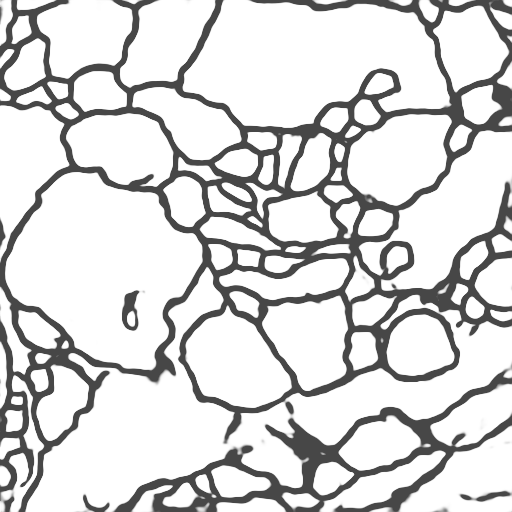
\includegraphics[scale=0.2]{figuras/2_predict.png}
    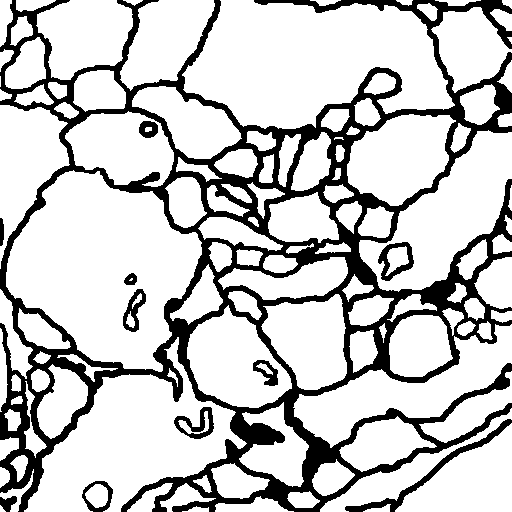
\includegraphics[scale=0.2]{figuras/2.png}
    \caption{Please look carefully at the two images. they are pretty the same, but wait, isn't the black in the left image not so black?}\label{fig:unetcomp}
\end{figure}

Hey! The network is not 100 percent sure about the prediction, so the output is possibility, which after converting to 0-255 uint8 value, is not 0 (pure black) nor 255 (pure white), but something in between. And the evaluation code requires that each pixel value to be the same as the label, to be count as a TP or TN. So if we want to use this code, we must conduct binarization on predictions before we compare pixels. Then we conduct experiment to select the optimal threshold of binarization, whose result in this case, is 87. See Figure~\ref{fig:unetthre} for details.
\begin{figure}[htpb]
    \centering
    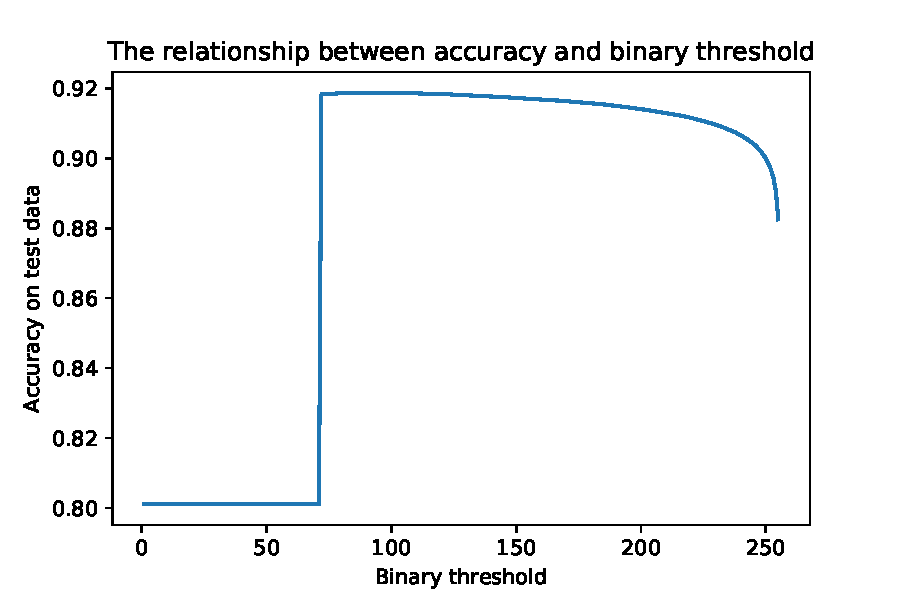
\includegraphics[scale=0.5]{figuras/unet_acc_thre.pdf}
    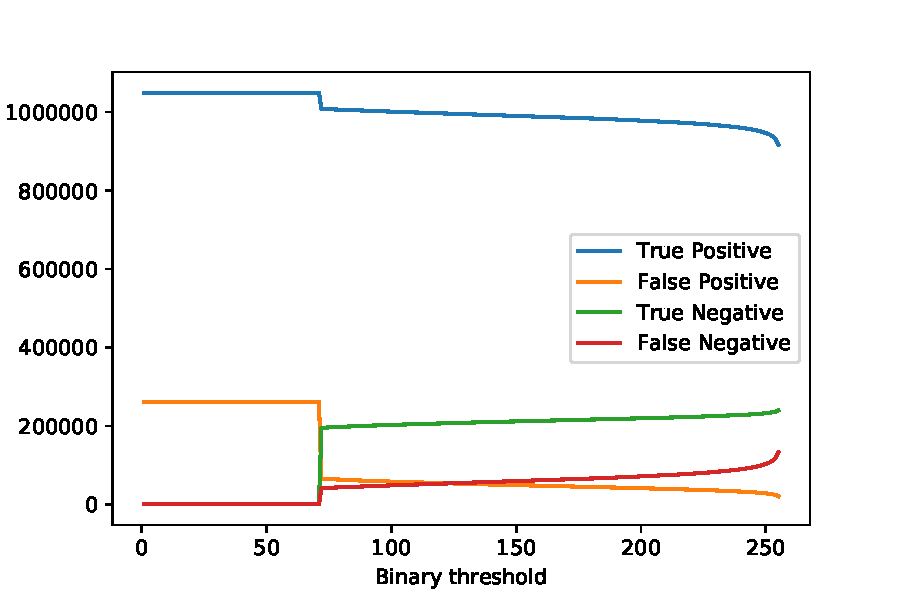
\includegraphics[scale=0.5]{figuras/unet_verbose_thre.pdf}
    \caption{Selecting optimal binarization threshold based on retrained model.}\label{fig:unetthre}
\end{figure}

Then using this threshold, we trained for more 5 epochs and Figure~\ref{fig:unethis} shows the performance and training epochs. The best accuracy is 0.9189. It seems not improving much while the epochs increase, this may be that there is too many steps (2000) in an epoch, and the work is pretty much done in the first epoch.
\begin{figure}[htpb]
    \centering
    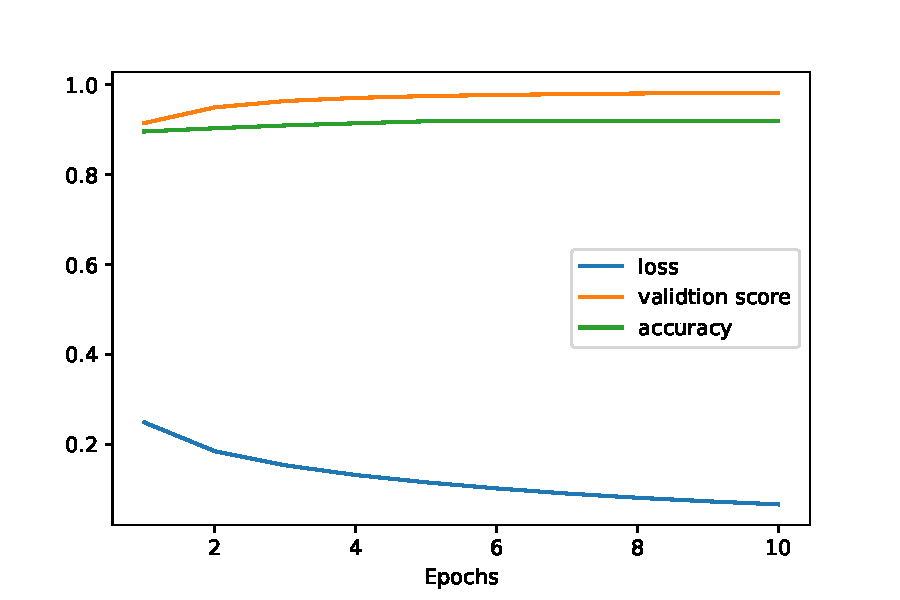
\includegraphics[scale=0.5]{figuras/unethistory.pdf}
    \caption{Training history of U-Net.}\label{fig:unethis}
\end{figure}